\chapter{信号处理初步}
\label{chap:signal-processing}

\begin{focusbox}{本章复习路线}
信号调理使传感器输出适合采集；数字信号处理则从有限数据中提取周期、时延、频率和功率分布。本章把第2章的傅里叶分析落实为可计算的分析流程：
\[
\text{采样与量化}\ \longrightarrow\ \text{有限记录与DFT}
\ \longrightarrow\ \text{相关分析}\ \longrightarrow\ \text{功率谱与互谱}.
\]
\textbf{学习目标：}能选择采样率与记录长度，解释混叠、泄漏和栅栏效应，按明确的时移约定求相关函数，并利用相关峰与功率谱完成测量分析。计算结果不仅要有数值，还应说明单位、归一化方法和适用条件。
\end{focusbox}

\begin{table}[H]
\centering\small
\begin{tabularx}{\linewidth}{@{}p{3cm} X@{}}
\toprule
复习模块 & 核心能力 \\
\midrule
数字化与采样 & 区分时间离散、幅值离散，判断混叠频率和抗混叠条件。 \\
有限记录与频谱 & 联系 $f_s,N,T,\Delta f$，区分泄漏、谱峰漏读和实际频率分辨能力。 \\
相关分析 & 区分相关、协方差、相关系数，判断时延方向与周期成分。 \\
功率谱分析 & 用谱面积核对均方值，正确使用单边谱、周期图和分段平均。 \\
互谱与相干 & 联系系统频响、输入输出关系与噪声，保留相位和统计条件。 \\
\bottomrule
\end{tabularx}
\end{table}

\section{从模拟信号到可计算的数字记录}

\subsection{信号处理的目的与基本链路}
信号处理主要服务于三个目标：分离有用信号与噪声，提取幅值、周期、时延等特征，以及补偿已知的测量系统误差。典型链路为
\[
\text{传感器}\ \longrightarrow\ \text{放大与模拟滤波}
\ \longrightarrow\ \text{采样、量化、编码}
\ \longrightarrow\ \text{数字分析与结果解释}.
\]
前置放大应使有效信号充分利用A/D量程，又不发生过载；模拟抗混叠滤波应在采样前限制带外成分。数字滤波、相关和谱分析在采集后进行，不能补救已经丢失的信息。

\dfn{采样、量化与编码}{\textbf{采样}在离散时刻读取模拟值，使时间离散；\textbf{量化}用有限个电平近似样本值，使幅值离散；\textbf{编码}把电平编号表示为数码。理想采样序列为
\[
x[n]=x(nT_s),\qquad T_s=\frac{1}{f_s},\qquad n\in\mathbb Z.
\]
只经过采样的序列，其样本幅值仍可连续取值；完成量化、编码后才得到有限字长的数字记录。}

\subsection{有限记录的四个基本参数}
采集 $N$ 个连续样本，取 $n=0,1,\ldots,N-1$，定义分析记录长度
\[
\boxed{T=NT_s=\frac{N}{f_s}},\qquad
\boxed{\Delta f=\frac{f_s}{N}=\frac{1}{T}}.
\]
这里 $T$ 是DFT对应的观察时长及周期延拓周期；第一点到最后一点的时间差为 $(N-1)T_s$。程序中应使用 $t_n=n/f_s$，不能把含首尾两端的 $N$ 个等分点误当成间隔为 $1/f_s$ 的样本。

\begin{table}[H]
\centering\small
\begin{tabularx}{\linewidth}{@{}l l X@{}}
\toprule
参数 & 单位 & 首先决定什么 \\
\midrule
$f_s$ & Hz & 采样频带；实信号基带分析上限为 $f_s/2$。 \\
$T_s$ & s & 相邻样本的时间间隔、整数样本时延的步长。 \\
$T$ & s & 观察多少周期，有限窗谱峰的宽度尺度。 \\
$N$ & 点数 & 在给定 $f_s$ 下决定记录时长与原始DFT频点间距。 \\
\bottomrule
\end{tabularx}
\end{table}

\Needspace{8cm}
\section{采样、混叠与量化误差}

\subsection{为什么频率会折叠}
\noindent\keypoint{复习重点：采样产生频谱周期复制；混叠使不同模拟频率得到同一个样本序列。}

由第2章的理想采样关系，
\[
X_s(f)=\frac{1}{T_s}\sum_{m=-\infty}^{\infty}X(f-mf_s).
\]
相邻复制谱若重叠，便不能从样本唯一辨认原频谱。对低通信号 $X(f)=0$（$|f|>f_m$），常用的无混叠充分条件为
\[
\boxed{f_s>2f_m}.
\]
$f_s/2$ 称为奈奎斯特频率或折叠频率。严格大于号为边界留出空间；恰好以两点采一个周期时，某些相位的正弦样本甚至全为零。

对于单个余弦，频率 $f_0$ 与 $f_0+mf_s$ 的样本一致；频率 $f_0$ 与 $-f_0$ 也不能仅凭实余弦样本区分。折叠到 $[0,f_s/2]$ 的频率可用
\[
\boxed{f_a=\min_{m\in\mathbb Z}|f_0-mf_s|},\qquad 0\leq f_a\leq f_s/2.
\]
对正弦或含初相位的信号，还须在折叠后核对符号和相位，不能只改频率而保留原表达式的所有其他部分。

\begin{center}
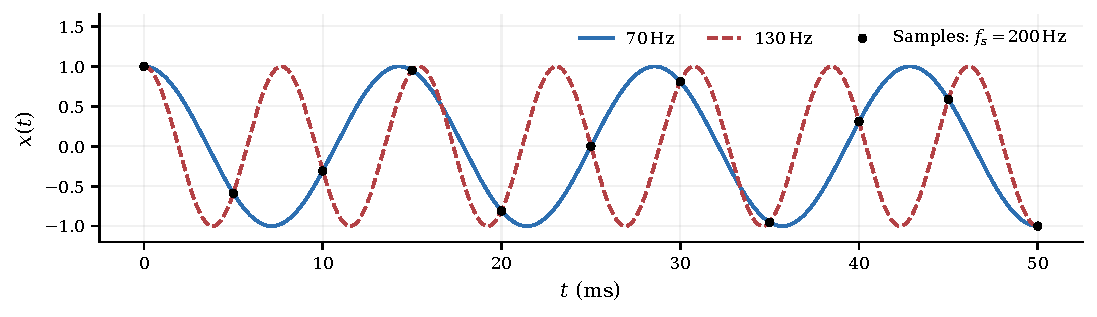
\includegraphics[width=.95\linewidth]{ch6-aliasing.pdf}
\end{center}
图中 $f_s=200\,\mathrm{Hz}$，$70\,\mathrm{Hz}$ 与 $130\,\mathrm{Hz}$ 余弦在每个采样点完全相同。较高频率的成分会被读成 $70\,\mathrm{Hz}$；延长记录只会增加同样的样本，不能消除此歧义。

\subsection{采样率与模拟抗混叠滤波怎样配合}
实际传感器输出可能同时含有目标频带内的信号、带外振动及宽带噪声。应先确定保留频带上限 $f_p$，再根据模拟滤波器的过渡带和所需阻带衰减选择 $f_s$。

\begin{itemize}
\item \textbf{采样前：}用模拟低通抑制可能折叠进目标频带的成分。截止频率、通带误差与阻带衰减应一起检查，不能只令截止频率等于 $f_s/2$。
\item \textbf{采样时：}使目标频带与复制频带之间留有过渡空间。$f_s$ 取最高目标频率的3至4倍可作为初步估计，最终仍取决于滤波器和误差要求。
\item \textbf{采样后：}数字滤波可继续抑制可辨认的噪声；已经折叠到目标频率上的成分与原信号混在一起，通常无法再分开。
\end{itemize}

\nt{增大 $f_s$ 有利于扩展无混叠频带，但在 $N$ 固定时会缩短 $T=N/f_s$、增大 $\Delta f$。选择采样率与选择记录长度是两个相互联系的设计问题。}

\subsection{量化步长、位数与编码}
\noindent\keypoint{复习重点：量程跨度决定每码代表多少输入量，量化误差界限以未过载、近邻舍入为前提。}

设ADC有 $b$ 位，共 $L=2^b$ 个码，完整输入跨度为 $D=x_{\max}-x_{\min}$。对将跨度分为 $L$ 个等宽区间的理想均匀量化器，
\[
\boxed{\Delta_q=\frac{D}{2^b}},\qquad
e_q[n]=x_q[n]-x[n],\qquad
\boxed{|e_q[n]|\leq\frac{\Delta_q}{2}}.
\]
误差界限对应近邻舍入且无过载的情形，端点行为按具体ADC规定处理。若把 $L$ 个重建电平安排为包含两端点的等间隔数列，则间距为 $D/(L-1)$；计算前必须统一量化器模型。

例如 $\pm5\,\mathrm{V}$ 表示 $D=10\,\mathrm{V}$，12位ADC常用的LSB为
\[
\Delta_q=\frac{10}{4096}\,\mathrm{V}\approx2.4414\,\mathrm{mV},
\qquad |e_q|\leq1.2207\,\mathrm{mV}.
\]
双极性输入可以采用偏移二进制或补码等编码；\textbf{不能仅因存在符号位，就把完整跨度内的码数一律减为 $2^{b-1}$。}每增加一位，理想步长约减半；增益设置合理也能改善输入折算的量化分辨力，但会减少过载余量。

若量化误差可近似为 $[-\Delta_q/2,\Delta_q/2]$ 上均匀分布且与信号弱相关，则其均方值约为 $\Delta_q^2/12$。这是噪声模型，不能保证每一条缓慢变化或周期样本记录都满足；实际准确度还受非线性、漂移与模拟噪声限制。

\Needspace{8cm}
\section{有限记录、窗函数与离散频谱}

\subsection{截断为什么产生频谱泄漏}
\noindent\keypoint{复习重点：时间相乘对应频率卷积；窗的主瓣与旁瓣影响的是不同方面。}

实际计算只能使用有限记录。以矩形窗保留 $0\leq t<T$ 内的数据，相当于
\[
x_T(t)=x(t)w_T(t),\qquad
W_T(f)=T\Sa(\pi fT)e^{-\iu\pi fT},\qquad \Sa u=\frac{\sin u}{u}.
\]
因此 $X_T(f)=X(f)*W_T(f)$。无限长正弦的理想线谱与窗谱卷积后变成有主瓣、旁瓣的谱形；原来集中于单一频率的成分扩散到其他频率，这称为\textbf{频谱泄漏}。

\textbf{主瓣宽度}决定相邻谱峰是否容易分开；\textbf{旁瓣高度及其衰减}决定强分量在较远频率处对弱分量的遮蔽程度。较低旁瓣通常要付出较宽主瓣的代价，没有对所有任务都最优的窗。

\begin{center}
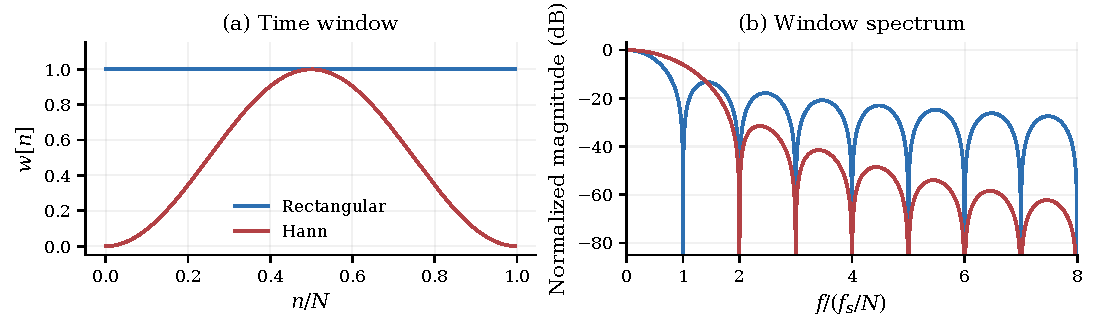
\includegraphics[width=.98\linewidth]{ch6-windows.pdf}
\end{center}
图中频率按 $\Delta f=f_s/N$ 归一化。矩形窗首个正频率零点约在 $\Delta f$，Hann窗约在 $2\Delta f$；图示只画主瓣的正半侧。

\begin{table}[H]
\centering\small
\begin{tabularx}{\linewidth}{@{}l c c X@{}}
\toprule
窗 & 主瓣零点间宽度 & 最高旁瓣约值 & 适用侧重 \\
\midrule
矩形窗 & $2/T$ & $-13\,\mathrm{dB}$ & 主瓣窄；适合相干采样及幅值相近的近邻成分。 \\
Hann窗 & $4/T$ & $-31\,\mathrm{dB}$ & 降低远处泄漏；较宽主瓣可能合并近邻谱峰。 \\
\bottomrule
\end{tabularx}
\end{table}
表中数值用于较长记录的常见窗形，幅度均相对窗谱峰值。离散Hann窗可取周期形式 $w[n]=\tfrac12-\tfrac12\cos(2\pi n/N)$；若用 $N-1$ 作分母，应相应计算实际窗的归一化量。

\subsection{DFT、频点位置与FFT}
对有限序列 $x[n]$，定义未归一化的 $N$ 点DFT
\[
\boxed{X_N[k]=\sum_{n=0}^{N-1}x[n]e^{-\iu2\pi kn/N}},\qquad
x[n]=\frac1N\sum_{k=0}^{N-1}X_N[k]e^{\iu2\pi kn/N}.
\]
第 $k$ 个频点为 $f_k=kf_s/N$，间距为 $\Delta f=f_s/N$。高于 $f_s/2$ 的DFT频点应解释为负频率，如 $k>N/2$ 时可写成 $(k-N)f_s/N$。实序列满足共轭对称 $X_N[N-k]=X_N^*[k]$。

\textbf{FFT是计算DFT的快速算法}，不会改变DFT定义、频点位置和有限记录固有的限制。DFT可以解释为有限序列周期延拓后的傅里叶级数系数乘 $N$；周期延拓是分析模型，并不表示真实信号必然每 $T$ 秒重复。

\Needspace{5cm}
\subsection{整周期截断、栅栏效应与加零}
若单频信号满足
\[
\boxed{f_0T=m\in\mathbb Z},\qquad f_0=m\Delta f,
\]
记录包含整数个周期，频率恰好落在DFT频点上，称为\textbf{相干采样}。对理想单频、矩形窗且无混叠的数据，能量只落在相应的一对DFT频点；在这些离散频点上没有向其他点泄漏。连续的有限窗频谱仍然有主瓣与旁瓣，不能因此说截断的影响已在所有频率上消失。

若 $f_0/\Delta f$ 不是整数，DFT只读取窗后连续谱的一组离散位置，可能错过谱峰，造成频率读数与峰值幅度偏差，称为\textbf{栅栏效应}。它与泄漏相关，但不是同一个问题：泄漏来自有限窗，栅栏效应来自频点有限。

\textbf{加零}是在 $N$ 个已采样数据后补零，计算 $M>N$ 点DFT。频点间距变为 $f_s/M$，可更密地显示同一条窗后频谱，改善峰位插值与读图。它没有增加观察时长，也没有使主瓣变窄，\textbf{不能提高原记录区分相邻频率的物理能力}。

\nt{有时把 $\Delta f=1/T$ 称为“频率分辨率”，准确含义首先是原始DFT频点间距。两频能否分开，还受窗的主瓣宽度、幅值差、噪声及判据影响。要提高实际分辨能力，通常要延长有效记录；不能只增加补零点数。}

\subsection{幅值谱的标定：先确认单双边与窗增益}
当 $x[n]=A\cos(2\pi mn/N+\theta)$ 且 $0<m<N/2$，相干矩形窗下
\[
|X_N[m]|=\frac{NA}{2},\qquad
\boxed{A=\frac{2|X_N[m]|}{N}}.
\]
直流点以及偶数 $N$ 时的奈奎斯特点没有独立的负频率配对，不乘2。其余正频率的单边幅值谱由双边幅值谱合并得到；对任意噪声频点，不宜直接把该数值解释为一条确定正弦的幅值。

使用窗 $w[n]$ 后，定义相干增益 $C_g=N^{-1}\sum_nw[n]$。对孤立、落点准确且远离直流与奈奎斯特频率的单频分量，幅值近似按
\[
A\approx\frac{2|X_w[m]|}{\sum_nw[n]}=\frac{2|X_w[m]|}{NC_g}
\]
校正；偏离频点时仍可能有峰值低估。\textbf{功率谱密度采用窗平方和归一化}，与这里的窗增益校正不同，不能混用。

\Needspace{8cm}
\section{相关分析：从相似程度到周期和时延}

\subsection{相关、协方差与相关系数}
\noindent\keypoint{复习重点：相关函数包含均值贡献；相关系数去均值、无量纲，衡量线性相关程度。}

对具有有限二阶矩的随机变量 $x,y$，定义
\[
\mu_x=\mathrm E[x],\quad \sigma_x^2=\mathrm E[(x-\mu_x)^2],\quad
C_{xy}=\mathrm E[(x-\mu_x)(y-\mu_y)].
\]
若 $\sigma_x\sigma_y>0$，相关系数为
\[
\boxed{\rho_{xy}=\frac{C_{xy}}{\sigma_x\sigma_y}},\qquad -1\leq\rho_{xy}\leq1.
\]
$\rho=1$ 或 $-1$ 表示完全正或负线性相关；$\rho=0$ 表示不相关，不排除非线性关系。例如对关于零对称的非退化随机变量 $x$，取 $y=x^2$，在相关矩存在时可有 $C_{xy}=0$，但 $y$ 显然由 $x$ 决定。

\nt{独立且二阶矩存在可推出不相关；一般不能反推独立。相关系数也不是因果证据。若方差为零，常数变量的相关系数因分母为零而无定义。}

\subsection{平稳条件与时间平均}
本章主要讨论\textbf{实值广义平稳过程}：均值不随时间变化，二阶矩有限，自相关仅与时间差有关。两个过程进行互相关与互谱分析时，还要求\textbf{联合广义平稳}，使交叉二阶统计量也仅依赖时间差。

\dfn{本章的相关函数与时移约定}{对实值平稳过程，取
\[
\boxed{R_x(\tau)=\mathrm E[x(t)x(t+\tau)]},\qquad
\boxed{R_{xy}(\tau)=\mathrm E[x(t)y(t+\tau)]}.
\]
相应的协方差函数为
\[
C_x(\tau)=R_x(\tau)-\mu_x^2,\qquad
C_{xy}(\tau)=R_{xy}(\tau)-\mu_x\mu_y.
\]
在非零方差下，$\rho_x(\tau)=C_x(\tau)/\sigma_x^2$、$\rho_{xy}(\tau)=C_{xy}(\tau)/(\sigma_x\sigma_y)$。}

满足相应遍历条件时，可以用单次充分长记录的时间平均代替总体平均，例如
\[
R_{xy}(\tau)=\lim_{T\to\infty}\frac1T\int_0^T x(t)y(t+\tau)\diff t.
\]
平稳性本身不保证遍历性；确定性周期信号则可直接按一周期做时间平均。对能量有限的脉冲，相关定义改为 $\int_{-\infty}^{\infty}x(t)y(t+\tau)\diff t$，\textbf{不除以趋于无穷的 $T$}，否则平均结果为零。

\subsection{自相关的性质与周期识别}
\begin{align*}
R_x(0)&=\mathrm E[x^2]=\sigma_x^2+\mu_x^2,\\
R_x(-\tau)&=R_x(\tau),\qquad |R_x(\tau)|\leq R_x(0),\\
\rho_x(0)&=1\quad(\sigma_x>0).
\end{align*}
因此零时移处是自相关的最大值之一，等于均方值；归一化相关系数才在零时移处等于1。相同波形按其周期平移仍相似，所以周期成分会在自相关中留下重复峰。

对 $x(t)=A\sin(\omega_0t+\varphi)$ 按时间平均，或令初相位在 $[0,2\pi)$ 上均匀随机，均有
\[
\boxed{R_x(\tau)=\frac{A^2}{2}\cos\omega_0\tau}.
\]
自相关保留该正弦的频率和幅值平方信息，丢失其绝对初相位。若 $x=s+n$，且 $s,n$ 互不相关、噪声均值为零，则 $R_x=R_s+R_n$；当噪声相关在较大时移处很小，周期峰就比原时域波形更易识别。

\begin{center}
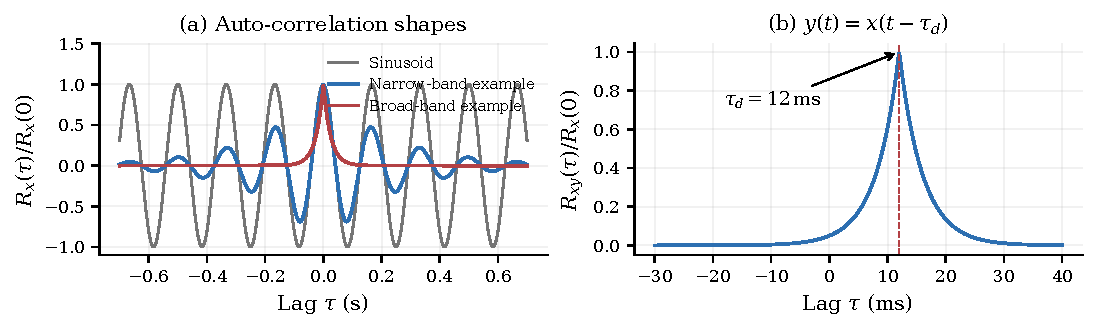
\includegraphics[width=.98\linewidth]{ch6-correlation.pdf}
\end{center}
左图用具体模型比较持续周期相关和衰减相关；带宽越宽，相关的集中时间尺度通常越短。右图表示正增益的延迟副本，其互相关峰位于正时延。

\nt{“随机信号的自相关随时移趋于零”不是普遍定律。只有去均值后的相关确实衰减时，才有 $R_x(\tau)\to\mu_x^2$；零均值时才趋于零。含随机相位正弦或持久相关成分的平稳过程可不衰减。}

\subsection{互相关的时延方向与工程解释}
实值联合平稳过程满足
\[
\boxed{R_{xy}(\tau)=R_{yx}(-\tau)},\qquad
|C_{xy}(\tau)|\leq\sigma_x\sigma_y.
\]
互相关一般既非奇函数也非偶函数，峰也可能恰在零时移处。为判断峰的正负方向，直接代入\textbf{延迟模型}
\[
y(t)=a\,x(t-\tau_d),\qquad a>0,
\]
得到
\[
\boxed{R_{xy}(\tau)=aR_x(\tau-\tau_d)}.
\]
所以 $y$ 比 $x$ 晚到 $\tau_d>0$，$R_{xy}$ 的主峰在 $\tau=+\tau_d$。若交换信号顺序，峰移到负侧；采用 $y(t-\tau)$ 的另一种定义时也会反号。使用软件之前应核对它的相关定义。

\begin{table}[H]
\centering\small
\begin{tabularx}{\linewidth}{@{}p{2.3cm} X@{}}
\toprule
应用 & 由相关峰到测量结果 \\
\midrule
运动测速 & 两探头沿运动方向相距 $d$，同一纹理依次通过，速度 $v=d/\tau_d$。 \\
传播测速 & 已知两接收位置间的传播路程差 $d$，由时延求传播速度 $c=d/\tau_d$。 \\
回波测距 & 发射与回波延迟是往返时间，目标距离 $L=c\tau_d/2$。 \\
周期诊断 & 由自相关非零重复峰间距估计周期，再与部件转速或故障特征频率比较。 \\
\bottomrule
\end{tabularx}
\end{table}
周期波形会产生相隔一个周期的多个相关峰，时延可能有整周期歧义；应结合允许时延范围或使用宽带非周期特征。相关峰的位置也会受有限记录、噪声和传播畸变影响。

\Needspace{4cm}
\textbf{两端接收的漏损定位：}设两接收器相距 $L$，漏点距第一接收器为 $s$，波速为 $c$。令 $x$、$y$ 分别为第一、第二接收器信号，则第二路相对第一路的到达时延为
\[
\tau_d=\frac{L-s}{c}-\frac{s}{c}=\frac{L-2s}{c},
\qquad \boxed{s=\frac{L-c\tau_d}{2}}.
\]
此处的2来自两条传播路程之差，与回波往返测距的几何原因不同；$\tau_d$ 的正负还指示漏点位于中点哪一侧。

\subsection{有限数据的相关估计}
对长度 $N$ 的实序列、非负整数时移 $\ell$，定义有效乘积和
\[
Q_{xy}[\ell]=\sum_{n=0}^{N-1-\ell}x[n]y[n+\ell],\qquad 0\leq\ell<N.
\]
两种常见估计为
\[
\widehat R_{xy}^{\,(b)}[\ell]=\frac{Q_{xy}[\ell]}{N},\qquad
\widehat R_{xy}^{\,(u)}[\ell]=\frac{Q_{xy}[\ell]}{N-\ell}.
\]
在联合平稳条件下，且使用未去均值的真相关定义时，前者期望为 $(1-\ell/N)R_{xy}[\ell]$，后者为 $R_{xy}[\ell]$，故分别称\textbf{有偏}和\textbf{无偏}估计。大时移下有效样本对减少，无偏估计的波动往往更大。有偏自相关估计适合构造非负周期图，但大时移受到更强压低。

若要估计协方差，先减均值；用同一有限记录估计均值后，上述“无偏”称呼不能保证协方差估计严格无偏。软件还可能使用全局能量或局部重叠能量归一化，需注明。换算实际时延时用 $\tau=\ell/f_s$；整数峰位的时间步长是 $T_s$，亚样本插值精度还取决于带宽和信噪比。

\Needspace{8cm}
\section{功率谱、互谱与频域测量}

\subsection{自功率谱密度与均方值}
\noindent\keypoint{复习重点：PSD给出每单位频宽的均方值分布；谱下面积才是功率。}

对实值广义平稳过程，若 $R_x(\tau)$ 绝对可积，维纳--辛钦关系为
\[
\boxed{S_x(f)=\int_{-\infty}^{\infty}R_x(\tau)e^{-\iu2\pi f\tau}\diff\tau},\qquad
R_x(\tau)=\int_{-\infty}^{\infty}S_x(f)e^{\iu2\pi f\tau}\diff f.
\]
$S_x(f)$ 为双边自功率谱密度，实、偶、非负；对含周期或直流的过程，也可用包含冲激谱线的广义谱描述。令 $\tau=0$ 得
\[
\boxed{\int_{-\infty}^{\infty}S_x(f)\diff f
=R_x(0)=\sigma_x^2+\mu_x^2=x_{\mathrm{rms}}^2}.
\]
若 $x$ 的单位为V，PSD单位为 $\mathrm{V^2/Hz}$，积分为 $\mathrm{V^2}$。此处“功率”通常指信号的均方值；电压在电阻 $R$ 上的电功率还应除以 $R$。

实信号的单边谱 $G_x(f)$ 将负频率功率合并到正侧：对普通连续谱 $f>0$，$G_x(f)=2S_x(f)$，并保持
\[
\int_0^\infty G_x(f)\diff f=x_{\mathrm{rms}}^2.
\]
直流谱线单独保留其全部权重；对离散频谱，直流点与偶数记录的奈奎斯特点不加倍。非零均值贡献 $\mu_x^2\delta(f)$；去均值后谱面积对应方差，而非原信号总均方值。

\subsection{幅值谱、能量谱和功率谱怎样区分}
\begin{table}[H]
\centering\small
\begin{tabularx}{\linewidth}{@{}p{2.4cm} p{3.3cm} X@{}}
\toprule
分析量 & 定义或尺度 & 应怎样解释 \\
\midrule
傅里叶幅度 & $|X(f)|$ & 连续变换的模，含时间单位；不等于PSD。 \\
单边谐波幅值 & 如 $2|X_N[k]|/N$ & 指定归一化下的正弦峰值，单位与原信号相同。 \\
能量谱密度 & $|X(f)|^2$ & 用于能量信号；积分等于 $\int|x(t)|^2\diff t$。 \\
功率谱密度 & $S_x(f)$ 或 $G_x(f)$ & 用于平稳功率分析；积分等于均方值。 \\
\bottomrule
\end{tabularx}
\end{table}

能量信号的Parseval关系为
\[
\int_{-\infty}^{\infty}|x(t)|^2\diff t
=\int_{-\infty}^{\infty}|X(f)|^2\diff f.
\]
无限持续的功率信号不能直接将无限长 $X(f)$ 的模平方当作普通函数。用有限记录变换 $X_T(f)$，再对 $|X_T(f)|^2/T$ 做适当的统计平均与极限，才与PSD联系起来；随机过程的单次原始周期图通常不会随记录增长而逐点稳定到真PSD。

\subsection{周期图估计与正确归一化}
对采样率 $f_s$、长度 $N$ 的记录，令
\[
X_w[k]=\sum_{n=0}^{N-1}w[n]x[n]e^{-\iu2\pi kn/N}.
\]
按Hz计的\textbf{双边周期图}为
\[
\boxed{\widehat S_x(f_k)=\frac{|X_w[k]|^2}{f_s\sum_{n=0}^{N-1}w^2[n]}}.
\]
矩形窗时分母为 $Nf_s$。单边谱将成对的正负频点合并，内部正频率乘2，直流与奈奎斯特点例外。写成 $|X_N|^2/N$ 时，频率及DFT归一化约定可能不同；\textbf{报告每Hz的PSD时不能遗漏 $f_s$}。

矩形窗下可用离散Parseval关系核对：
\[
\boxed{\sum_{k=0}^{N-1}\widehat S_x(f_k)\Delta f
=\frac1N\sum_{n=0}^{N-1}|x[n]|^2}.
\]
一般窗的右侧变成 $\sum_nw^2[n]|x[n]|^2/\sum_nw^2[n]$。若补零到 $M$ 点，周期图分母仍用实际窗的 $f_s\sum w^2$，积分步长改为 $f_s/M$；不能把补零点也算进有效记录能量归一化。

\subsection{分段平均：方差与分辨能力的折中}
单条有限记录的周期图起伏很大。把平稳记录分为 $q$ 段，各自求周期图再平均：
\[
\boxed{\widehat G_{\mathrm{avg}}(f)=\frac1q\sum_{i=1}^{q}\widehat G_i(f)}.
\]
当各段估计近似独立且方差相同时，平均后的方差约为单段方差的 $1/q$，标准差约降为 $1/\sqrt q$。固定总时长时，段数越多，单段越短、主瓣越宽，实际频率分辨能力就越差。

\begin{center}
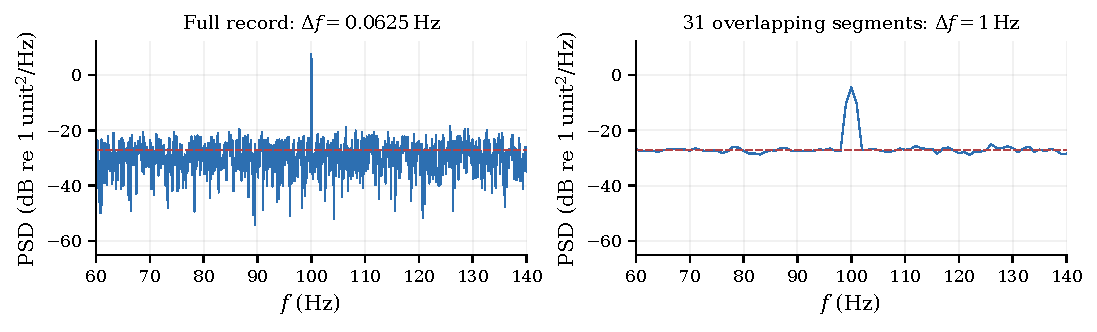
\includegraphics[width=.98\linewidth]{ch6-psd-average.pdf}
\end{center}
图示为相同16秒记录：长记录保留更尖的谱峰，1秒分段平均使噪声谱更平滑，但谱峰变宽。虚线为所加白噪声的理论单边PSD，原始噪声方差为1。

加窗并允许相邻段重叠的分段平均常称为Welch方法。Hann窗配合50\%重叠是常见选择；重叠使各段相关，实际独立平均数小于段数，不能机械套用方差恰好除以 $q$。选参时先按分辨要求确定\textbf{段长}，再按统计稳定性确定总时长与平均次数。瞬变、转速变化或工况切换需分段定位分析，整段平均可能掩盖变化。

\subsection{互谱、频率响应与相干函数}
沿用 $R_{xy}(\tau)=\mathrm E[x(t)y(t+\tau)]$，互功率谱密度定义为
\[
S_{xy}(f)=\int_{-\infty}^{\infty}R_{xy}(\tau)e^{-\iu2\pi f\tau}\diff\tau,
\qquad S_{yx}(f)=S_{xy}^*(f).
\]
互谱一般为复数，保留输入输出之间的相位关系。相同窗与采样约定下，其有限记录估计为
\[
\widehat S_{xy}(f_k)=\frac{X_w^*[k]Y_w[k]}{f_s\sum_{n=0}^{N-1}w^2[n]}.
\]
计算前后应保持相同的相关顺序。

对稳定LTI系统，若输出仅为输入响应，记 $H(f)=H(\iu2\pi f)$，则
\[
\boxed{S_y(f)=|H(f)|^2S_x(f)},\qquad
\boxed{S_{xy}(f)=H(f)S_x(f)}.
\]
前式给出幅值比 $|H|=\sqrt{S_y/S_x}$，但不能给出相位；后式在 $S_x>0$ 处可求复频响 $H=S_{xy}/S_x$。若 $y=h*x+n$ 且输出噪声 $n$ 与输入不相关，则
\[
S_y=|H|^2S_x+S_n,\qquad S_{xy}=HS_x.
\]
因此直接用自谱比会把输出噪声也算进去，互谱估计仍能提取与输入线性相关的响应；输入测量噪声则需另行分析。

\dfn{幅值平方相干函数}{在 $S_x(f)S_y(f)>0$ 处，
\[
\boxed{\gamma_{xy}^2(f)=\frac{|S_{xy}(f)|^2}{S_x(f)S_y(f)}},\qquad
0\leq\gamma_{xy}^2(f)\leq1.
\]
它衡量该频率上两信号的线性关联程度。对上述不相关输出噪声模型，
\[
\gamma_{xy}^2(f)=\frac{|H|^2S_x}{|H|^2S_x+S_n}.
\]
在此模型下，它等于输出功率中由输入线性响应贡献的比例。}

低相干可能来自其他输入、噪声、非线性、时变或估计误差，不能单独定位原因；高相干也不能证明因果方向。\textbf{估计相干性必须先对自谱、互谱做分段平均或等效平滑，再取比值}；单个未平均频点的 $|X^*Y|^2/(|X|^2|Y|^2)$ 恒为1，不能据此判断真实关联。
